\documentclass[16pt,aspectratio=169]{beamer}
\usetheme{polima}
\beamertemplatenavigationsymbolsempty

\usepackage[absolute,overlay]{textpos}
\usepackage[texcoord,gridcolor=red!10,subgridcolor=green!10,gridunit=mm]
{eso-pic}
\usepackage[dvipsnames]{xcolor}
\usepackage{animate}
\usepackage{tikz}
\usepackage{multirow} 
\usepackage{amsmath}
\usepackage{chemformula}
\usepackage{subcaption}
\usepackage[most]{tcolorbox}
\usepackage{empheq}
\usepackage{bm}
\usefonttheme{professionalfonts}
\usepackage{physics}
\usepackage[disablemarkdown]{pdfpc}
\usepackage{blkarray}

\newsavebox\CBox
\newcommand\hcancel[2][0.5pt]{%
  \ifmmode\sbox\CBox{$#2$}\else\sbox\CBox{#2}\fi%
  \makebox[0pt][l]{\usebox\CBox}%  
  \rule[0.25\ht\CBox-#1/2]{\wd\CBox}{#1}}

\newcommand\inbox[2][0.5pt]{%
  \ifmmode\sbox\CBox{$#2$}\else\sbox\CBox{#2}\fi%
  \makebox[0pt][l]{\usebox\CBox}{\wd\CBox}{#1}}

\newcommand<>{\slidehcancel}[1]{\alt#2{\hcancel{#1}\vphantom{#1}}{#1}}

\useinnertheme[rounded]{tcolorbox}

\tcbset{
  attach boxed title to top center={yshift=-2mm},
  enhanced,
  bottom=1mm
}

\usepackage{fontspec}

\setsansfont[
  Path           = ./fonts/klavika/,
  BoldFont       = Klavika_Bold.otf,
  ItalicFont     = Klavika_Regular_Italic.otf,
  BoldItalicFont = Klavika_Bold_Italic.otf]
  {Klavika_Regular.otf}
\setmonofont[
  Scale          = 0.9,
  Path           = fonts/,
  BoldFont       = consolab.ttf,
  ItalicFont     = consolai.ttf,
  BoldItalicFont = consolaz.ttf]
  {consola.ttf}

\usepackage{tikz}
\usetikzlibrary{decorations.pathmorphing}
\usetikzlibrary{decorations.markings}
\usetikzlibrary{shapes.geometric}
\usetikzlibrary{cd}
\usetikzlibrary{positioning}
\usetikzlibrary{chains}
\usetikzlibrary{mindmap}
\usetikzlibrary{positioning,patterns,arrows,shapes,shapes.arrows,arrows,intersections,shadows,backgrounds,snakes}
\usetikzlibrary{arrows.meta, decorations.text}
\usetikzlibrary{overlay-beamer-styles}

\definecolor{brass}{rgb}{0.71, 0.65, 0.26}

\newcommand{\pnl}[1]{\textbf{#1}}


\newcounter{mybox}
\newcommand\tikzmark[1]{%
  \tikz[remember picture,overlay] \node[inner xsep=0pt] (#1) {};
}
\newcommand<>\ColorBox[2][]{%
\stepcounter{mybox}%
\node[draw=red!70!black,fill=red!20,align=left,#1] (box\themybox) {#2};
}

\input{shortcuts.tex}

\newcommand\occasion{Ph.D.~Defense}

% the presentation starts here
\title[Optical Properties of 2D Semiconductors]{Optical Properties of Two-dimensional Semiconductors:\\Excitonic and Polaritonic Effects}
%
\author[Pedro A.~C.~Ninhos]{Pedro António Correia Ninhos}
%
\institute{POLIMA: Center for Polariton--driven Light--Matter Interactions\\ University of Southern Denmark\\
\textcolor{blue}{peni@mci.sdu.dk}}
%
\date{22-01-2026}

\AtBeginSection[]
{
    \begin{frame}<beamer>
    \frametitle{Outline}
    \tableofcontents[
        currentsection,
        sectionstyle=show/shaded,
        subsectionstyle=show/show/hide
    ]
    \end{frame}
}

\makeatletter
\setbeamertemplate{block title}{
    \begin{beamercolorbox}[wd=\textwidth,sep=0.8ex,center]{block title}
        \usebeamerfont*{block title}\insertblocktitle
    \end{beamercolorbox}
}
\makeatother

\begin{document}
\selectlanguage{english}

% title page
\begin{frame}
\only<1->{
\titlepage
}

\begin{textblock*}{8.0cm}(0.4cm,5.7cm)
Supervisors:\\
\small \, Prof.~N.~Asger Mortensen\\
\, Prof.~Nuno M.~R.~Peres\\
\, Prof.~Christos~Tserkezis\\
\normalsize Secondment Host:\\
\small \, Prof.~Juan~José~Palacios
\end{textblock*}

\end{frame}

%%%%%%%%%%%%%%%%%%%%%%%%%%%%%%%%%%%%%%%%%%%%%%%%%%%

\begin{frame}{Outline}
  \tableofcontents
\end{frame}

%!TEX root = ../main.tex %
% !TeX spellcheck = en_US

%%%%%%%  INTRODUCTION  %%%%%%%%%

\section{Introduction to Excitons in 2D Materials}
%%%%%%%%%%%%%%%%%%%%%%%%%%%%%%%%%%%%%%%%%%%%%%%%%%%%%%%%%%%%%%%%%%%%

% \begin{frame}{Optical Excitations in Matter}
%     \centering
%     
\begin{tikzpicture}[mindmap, grow cyclic, every node/.style=concept, concept color=blue!40!white,
    level 1/.append style={level distance=3.5cm,sibling angle=120},
    level 2/.append style={level distance=2.8cm,sibling angle=45},
    level 3/.append style={level distance=2cm,sibling angle=40},
    every annotation/.style={fill=red!20}]
    \tikzset{every node/.append style={scale=0.8}}
\node [concept,scale=1.0] (center) {\Large Solid Materials}

    child [concept color = violet!60!white,grow=-150] {
        node[alt=<{2}>{circular glow={fill=brass}}{}] (metals) {Metals} 
            child[visible on=<3->,grow=120] { node[alt=<{3}>{circular glow={fill=brass}}{}] {Free charges}}
            child[visible on=<4->,grow=180] { node[alt=<{4}>{circular glow={fill=brass}}{}] {Conducting}}
            child[visible on=<5->,grow=-120] { node[alt=<{5}>{circular glow={fill=brass}}{}] {Plasmons}}}
    child [concept color = red!60!white,grow=-30] { 
        node[alt=<{6}>{circular glow={fill=brass}}{}] (dielectrics) {Dielectric}
            child[visible on=<7->,grow=60] { node[alt=<{7}>{circular glow={fill=brass}}{}] {Bound charges}}
            child[visible on=<8->,grow=0] { node[alt=<{8}>{circular glow={fill=brass}}{}] {Insulating}}
            child[visible on=<9->,grow=-60] { node[alt=<{9}>{circular glow={fill=brass}}{}] {Excitons}}
    };

    %\path (center) to[circle connection bar switch color=from (blue!40!white) to (violet!60!white)] (metals);
    % \node [right,text width=5.2cm, minimum width = 5.2cm,visible on=<3->] at (metals.south west)
    %     {Free charge };
    % \path (center) to[circle connection bar switch color=from (blue!40!white) to (red!60!white)] (dielectrics);
    % \node [annotation,right,text width=8.cm, minimum width = 8.cm,visible on=<5->] at (dielectrics.south east)
    %     {Excitons};

\end{tikzpicture}

% \end{frame}

\begin{frame}{Optical Excitations in Matter}
   \centering
    



\tikzset{every picture/.style={line width=0.75pt}} %set default line width to 0.75pt        

\begin{tikzpicture}[x=0.75pt,y=0.75pt,yscale=-1,xscale=1,remember picture]
%uncomment if require: \path (0,300); %set diagram left start at 0, and has height of 300
\draw[lightgray,thin,dashed] (60,30)  grid  (500,250);
\useasboundingbox (60,20) rectangle (500,255);

\begin{scope}[yshift={9.5}]
    %\fill[fill=blue!10] (60,30) rectangle (500,250);
%Shape: Brace [id:dp45369403742662895] 
\draw<2->   (200,56) .. controls (195.33,56.01) and (193,58.34) .. (193.01,63.01) -- (193.09,129.51) .. controls (193.1,136.18) and (190.77,139.51) .. (186.1,139.52) .. controls (190.77,139.51) and (193.1,142.84) .. (193.11,149.51)(193.11,146.51) -- (193.2,216.01) .. controls (193.2,220.68) and (195.53,223.01) .. (200.2,223) ;
%Shape: Brace [id:dp9306672772670488] 
\draw<5->   (309,46) .. controls (304.33,46) and (302,48.33) .. (302,53) -- (302,73.25) .. controls (302,79.92) and (299.67,83.25) .. (295,83.25) .. controls (299.67,83.25) and (302,86.58) .. (302,93.25)(302,90.25) -- (302,113.5) .. controls (302,118.17) and (304.33,120.5) .. (309,120.5) ;
%Shape: Brace [id:dp8400849826669508] 
\draw<9->   (309,162) .. controls (304.33,162) and (302,164.33) .. (302,169) -- (302,189.25) .. controls (302,195.92) and (299.67,199.25) .. (295,199.25) .. controls (299.67,199.25) and (302,202.58) .. (302,209.25)(302,206.25) -- (302,229.5) .. controls (302,234.17) and (304.33,236.5) .. (309,236.5) ;

% \draw (200.,87.) -- (340,87.);
% \draw (200.,203.0) -- (340,203.0);

% Text Node
\draw<1-> (60,130) node [anchor=north west][inner sep=0.75pt]  [font=\Large] [align=left] {Solid Materials};
% Text Node
\draw<3-> (215.4,74.) node [anchor=north west][inner sep=0.75pt]  [font=\large] [align=left] {Metals};
% Text Node
\draw<4-> (210,190.0) node [anchor=north west][inner sep=0.75pt]  [font=\large] [align=left] {Dielectrics};
% Text Node
\draw<6-> (313,42.0) node [anchor=north west][inner sep=0.75pt]   [align=left] {Free charges};
% Text Node
\draw<7-> (313.6,75.) node [anchor=north west][inner sep=0.75pt]   [align=left] {Conducting};
% Text Node
\draw<8-> (314.4,110) node [anchor=north west][inner sep=0.75pt]   [align=left] {Plasmons};
% Text Node
\draw<10-> (314,158.6) node [anchor=north west][inner sep=0.75pt]   [align=left] {Bound charges};
% Text Node
\draw<11-> (313.6,191.0) node [anchor=north west][inner sep=0.75pt]   [align=left] {Insulating};
% Text Node
\draw<12-> (314.2,225.0) node [anchor=north west][inner sep=0.75pt]   [align=left] {Dipolar excitations (excitons)};
\end{scope}

\end{tikzpicture}
\end{frame}

\subsection{Context}

\begin{frame}{Excitons in photonics}

\begin{textblock*}{5.0cm}(0.2cm,1.2cm)
Relevant for:
\end{textblock*}

\begin{textblock*}{5.0cm}(0.2cm,2.0cm)
    \,\,\,\,\,\,\, {\color<2>{red} Light--matter interactions}
    \begin{figure}
        \includegraphics[scale=0.3]{Figures/light_matter.png}
    \end{figure}
    \,\,\,\,\,\,\, \small J. Shang et al. - \textit{ACS Photonics} \\ 
    \hspace{1.4cm} \textbf{10} 7 (2023)
    % mainly in 2D dimensions, constitute a playground to study light−matter interactions, many-body effects and their applications in photonics
\end{textblock*}

\begin{textblock*}{5.0cm}(5.2cm,2.0cm)
    \,\,\,\,\,\,\, {\color<3>{red}Quantum Light Sources}
    \begin{figure}
        \includegraphics[scale=0.25]{Figures/photon_emission.png}
    \end{figure}
    \,\,\,\,\,\,\, \small S. Fiedler et al. - \textit{2D Mater.} \\ 
    \hspace{1.6cm} \textbf{10} 021002 (2023)
    % tunable photon emission from 2D semiconductors
\end{textblock*}

\begin{textblock*}{5.0cm}(10.5cm,2.0cm)
    \,\,\,\,\,\,\,\,\,\,\, {\color<4>{red}Valleytronics}
    \begin{figure}
        \includegraphics[scale=0.3]{Figures/communications.png}
    \end{figure}
    \,\,\,\,\,\,\, \small Yi Zhu et al. - \textit{Nano Letters} \\
    \hspace{1.8cm} \textbf{25} 21 (2025)
    % improve optical communication systems
\end{textblock*}


\end{frame}

\begin{frame}{Excitons in two-dimensional materials}
        \begin{columns}[T]

            \column{.5\linewidth}
            \onslide<1->{
                \textbf{For a typical 3D material (e.g., GaAs)}
                \begin{equation*}
                    \begin{aligned}
                        E_{b,n} &= - \frac{R^*}{n^2} \\
                        R^*     &= \frac{2 \mu_{eh}^2 e^4}{\hbar^2 (8 \pi \varepsilon \varepsilon_0)^2}
                    \end{aligned}                   
                \end{equation*}
            }
            \column{.5\linewidth}
            \onslide<2->{
                \textbf{\,\,\,\,\, But for a 2D (insulating) material}

                \begin{figure}
                    \centering
                    \includegraphics[scale=1.]{Figures/hBN_permittivity.pdf}
                \end{figure}
            }
            
        \end{columns}


        \begin{columns}[T]

            \column{.6\linewidth}
            \begin{textblock*}{10.0cm}(0.cm,5.0cm)            
                \only<4->{
                    \vspace{-0.5cm}
                    \hspace{-0.5cm}
                    \begin{figure}
                        \includegraphics[scale=0.4]{Figures/Exciton_Series_b}
                    \end{figure}
                    \vspace{-0.4cm}
                    A. Chernikov et al. - \textit{Phys. Rev. Lett.} \textbf{113} 076802 (2014)
                }
            \end{textblock*}
%            \only<5>{
%                \begin{itemize}
%                    \item "Theoretical Methods for Excitonic Physics in 2D Materials", Maurício et al. Phys. Status Solidi B, 259: 2200097, 2022 \small (tutorial for exciton calculation methods)
%                    \item "Diele. screening in 2D insu.: Implications for excitonic and impurity states in graphane", Cudazzo et al., Phys. Rev. B \textbf{84}, 085406, 2011 \small (classical model for $\varepsilon(q)$)
%                \end{itemize}
%            }
            
            \column{.4\linewidth}
            \onslide<3->{
                \begin{itemize}
                    \item Excitonic series $\neq$ Rydberg series
                    \item Dielectric "constant" $\varepsilon = \lim_{q \to 0} \lim_{\omega \to 0} \varepsilon (q, \omega) = 1$
                    \item $\varepsilon (q)$ highly dependent on $q$ (non-locality)
                \end{itemize}
            }
            

        \end{columns}

\end{frame}

\subsection{Motivation}
%%%%%%%%%%%%%%%%%%%%%%%%%%%%%%%%%%%%%%%%%%%%%%%%%%%%%%%%%%%%%%%%%%%%

\begin{frame}{Hexagonal boron nitride in photonics}

\only<1->{
\begin{textblock*}{8.0cm}(0.2cm,1.5cm)
\begin{itemize}
    \item Low defects density [1] %People realized that Luminescent defect centers in hBN were a promising source for SPEs. Defects in hBN are known to reduce phonon lifetimes, and, thus, are detrimental to its use for IR nanophotonics, but such defects are at the heart of hBN’s promise as a single-photon emitter.
    \item Ballistic transport  in graphene [2] %as an encapsulating material, hBN enhances carriers mobility in graphene. This reports ballistic transport up to 28 micrometer
    \item Hyperbolic material (MIR) [3]
    \item Polaritonics in the MIR [4] %hBN interesting on its own as the active material. In this experimental work phonon-polaritons were excited. They used s-snom to measure the propagation length of phonon-polaritons.
\end{itemize}
\end{textblock*}


\begin{textblock*}{5.0cm}(6.8cm,1.cm)
\begin{figure}
    \centering
    \includegraphics[scale=0.5]{Figures/ballistic_transport.PNG}
\end{figure}
\end{textblock*}

\begin{textblock*}{5.0cm}(7.7cm,2.5cm)
[2]
\end{textblock*}

\begin{textblock*}{5.0cm}(10.4cm,1.1cm)
\begin{figure}
    \centering
    \includegraphics[scale=0.3]{Figures/phonon_polaritons.PNG}
\end{figure}
\end{textblock*}

\begin{textblock*}{5.0cm}(12.5cm,2.4cm)
[4]
\end{textblock*}

\begin{textblock*}{5.0cm}(.2cm,3.5cm)
\begin{figure}
    \centering
    \includegraphics[scale=0.3]{Figures/hBN_on_quartz.PNG}
\end{figure}
\end{textblock*}

\begin{textblock*}{5.0cm}(9cm,3.0cm)
\begin{figure}
    \centering
    \includegraphics[scale=0.4]{Figures/PL_hBN.PNG}
\end{figure}
\end{textblock*}

\begin{textblock*}{5.0cm}(2.cm,7.0cm)
[5,6]
\end{textblock*}

\begin{textblock*}{5.0cm}(9.7cm,4.5cm)
[5,6]
\end{textblock*}

\begin{textblock*}{8.0cm}(.2cm,7.5cm)
\scriptsize{[1] I.~H. Abidi et al. - \textit{Adv. Opt. Mater.} \textbf{7} 1900397 (2019)} \\
\scriptsize{[2] L. Banszerus et al. - \textit{Nano Lett.} \textbf{16} 1387--1391 (2016)} \\
\scriptsize{[3] J.~D. Caldwell et al. - \textit{Nat. Rev. Mat.} \textbf{4} 5221 (2019)}
\end{textblock*}
\begin{textblock*}{14.0cm}(7.0cm,7.5cm)
\scriptsize{[4] D. Rizzo et al. - \textit{Nano Lett.} \textbf{23} 8426--8435 (2023)} \\
\scriptsize{[5] J. Henriques et al. - \textit{J. Phys.: Cond. Matter} \textbf{32} 025304 (2019)} \\
\scriptsize{[6] C. Elias et al. - \textit{Nat. Comm.} \textbf{10} 2639 (2019)} %Colla between Laboratory Charles Coulomb Montpellier and Nottingham
\end{textblock*}

}
\end{frame}

\begin{frame}{Motivation}    
    \begin{columns}[T]

        \column{.5\linewidth}
        
            \begin{textblock*}{\linewidth}(0.3cm,1.1cm)
            
            \onslide<1->{
                \textbf{Rytova--Keldysh model} \only<7->{\textcolor{ForestGreen}{What can we do with it?}}
                \begin{equation*}
                    \varepsilon_{\mathrm{RK}} (q) = 1 + r_0 q \,\,, V_{\mathrm{RK}} (q) = \frac{e^2}{2 \varepsilon_0 q\varepsilon_{\mathrm{RK}} (q)}
                \end{equation*}}
                \only<2->{\begin{equation*}
                    V_{\mathrm{RK}} (r) = \frac{e^2}{4\pi\varepsilon_0}\frac{\pi}{2 r_0} \! \left[ \mathbf{H}_0\!\left(\frac{r}{r_0}\right)-Y_0\!\left(\frac{r}{r_0}\right)\right]
                \end{equation*}
            
                \begin{itemize}
                    \item Intuitive
                    \item Analytical expression
                \end{itemize}}
            \onslide<3->{
                \begin{itemize}
                    \item \textcolor{red}{Excitons are determined numerically}
                    \item \textcolor{red}{Questionable for layered systems}
                    \item \textcolor{red}{Screening parameter $r_0$ obtained from \textit{ab initio} methods either way}
                \end{itemize}
            }
            \end{textblock*}
        \column{.5\linewidth}
            \begin{textblock*}{\linewidth}(\linewidth+0.6cm,1.1cm)
                \onslide<4->{
                \textbf{Full numerical \textit{ab initio}} \only<8->{\textcolor{ForestGreen}{Can we optimize?}}
                    \begin{equation*}
                        \varepsilon_{\vectormath{G} \vectormath{G}'} (\vectormath{q}) = \delta_{\vectormath{G} \vectormath{G}'} - v_c(\vectormath{q} + \vectormath{G}) \chi^0_{\vectormath{G} \vectormath{G}'}(\vectormath{q})
                    \end{equation*}}
                \onslide<5->{
                    \begin{itemize}
                        \item Works for any kind of system
                        \item Several packages available (BerkeleyGW, Yambo, VESPA, etc...)
                        \item Captures screening in its $q$ entirety
                    \end{itemize}}
                \onslide<6->{
                    \begin{itemize}
                        \item \textcolor{red}{Computationally heavy}
                        \item \textcolor{red}{Physics harder to grasp}
                        \item \textcolor{red}{Codes are designed for 3D systems}
                    \end{itemize}
                }
            \end{textblock*}
    \end{columns}
\end{frame}

%!TEX root = ../main.tex %
% !TeX spellcheck = en_US

%%%%%%%  hBN Superlattice  %%%%%%%%%

\section{Part I: Exciton--Polaritons in a 1D hBN superlattice}
%%%%%%%%%%%%%%%%%%%%%%%%%%%%%%%%%%%%%%%%%%%%%%%%%%%%%%%%%%%%%%%%%%%%

\begin{frame}{Motivation}
    No motivation whatsoever
\end{frame}

\subsection{Hexagonal boron nitride in photonics}
%%%%%%%%%%%%%%%%%%%%%%%%%%%%%%%%%%%%%%%%%%%%%%%%%%%%%%%%%%%%%%%%%%%%

\begin{frame}{hBN in photonics}

\only<1->{
\begin{textblock*}{8.0cm}(0.2cm,1.5cm)
\begin{itemize}
    \item Low defects density [1] %People realized that Luminescent defect centers in hBN were a promising source for SPEs. Defects in hBN are known to reduce phonon lifetimes, and, thus, are detrimental to its use for IR nanophotonics, but such defects are at the heart of hBN’s promise as a single-photon emitter.
    \item Ballistic transport  in graphene [2] %as an encapsulating material, hBN enhances carriers mobility in graphene. This reports ballistic transport up to 28 micrometer
    \item Hyperbolic material (MIR) [3]
    \item Polaritonics in the MIR [4] %hBN interesting on its own as the active material. In this experimental work phonon-polaritons were excited. They used s-snom to measure the propagation length of phonon-polaritons.
\end{itemize}
\end{textblock*}


\begin{textblock*}{5.0cm}(6.8cm,1.cm)
\begin{figure}
    \centering
    \includegraphics[scale=0.5]{Figures/ballistic_transport.PNG}
\end{figure}
\end{textblock*}

\begin{textblock*}{5.0cm}(7.7cm,2.5cm)
[2]
\end{textblock*}

\begin{textblock*}{5.0cm}(10.4cm,1.1cm)
\begin{figure}
    \centering
    \includegraphics[scale=0.3]{Figures/phonon_polaritons.PNG}
\end{figure}
\end{textblock*}

\begin{textblock*}{5.0cm}(12.5cm,2.4cm)
[4]
\end{textblock*}

\begin{textblock*}{5.0cm}(.2cm,3.5cm)
\begin{figure}
    \centering
    \includegraphics[scale=0.3]{Figures/hBN_on_quartz.PNG}
\end{figure}
\end{textblock*}

\begin{textblock*}{5.0cm}(9cm,3.0cm)
\begin{figure}
    \centering
    \includegraphics[scale=0.4]{Figures/PL_hBN.PNG}
\end{figure}
\end{textblock*}

\begin{textblock*}{5.0cm}(2.cm,7.0cm)
[5,6]
\end{textblock*}

\begin{textblock*}{5.0cm}(9.7cm,4.5cm)
[5,6]
\end{textblock*}



\begin{textblock*}{8.0cm}(.2cm,7.5cm)
\scriptsize{[1] I.H. Abidi et al., \textit{Adv. Opt. Mater.} 7, 1900397 (2019)} \\
\scriptsize{[2] L. Banszerus et al., \textit{Nano Lett. } 16, 1387–1391 (2016)} \\
\scriptsize{[3] J. D. Caldwell et al., \textit{Nat. Rev. Mat.} 4, 5221 (2019)}
\end{textblock*}
\begin{textblock*}{14.0cm}(7.0cm,7.5cm)
\scriptsize{[4] D. Rizzo et al., \textit{Nano Lett. } 23, 18, 8426–8435 (2023)} \\
\scriptsize{[5] J. Henriques et al., \textit{J. Phys.: Cond. Matter} 32, 025304 (2019)} \\
\scriptsize{[6] C. Elias et al., \textit{Nat. Comm.} 10, 2639 (2019)} %Colla between Laboratory Charles Coulomb Montpellier and Nottingham
\end{textblock*}

}

\end{frame}

\subsection{Setup}


%%%%%%%%%%%%%%%%%%%%%%%%%%%%%%%%%%%%%%%%%%%%%%%%%%%%%%%%%%%%%%%%%%%

\begin{frame}[t]
\frametitle{hBN under an external periodic potential}


\begin{columns}[T]

        \column{.6\linewidth}
        \only<1->{
            \begin{textblock*}{10.0cm}(0.2cm,0.5cm)
            \begin{figure}
                \includegraphics[scale=0.8]{Figures/Work_on_hBN_perspective_2.pdf}
            \end{figure}
            \small
            ``Tunable Exciton Polaritons in Band-Gap Engineered hBN'' \\
            \underline{P.~Ninhos}, C.~Tserkezis, N.~A.~Mortensen, N.~M.~R.~Peres, ACS Nano  18, 31, (2024)
            \end{textblock*}
            
            }

        \column{.4\linewidth}

        \only<2->{
            \begin{textblock*}{4.0cm}(10.0cm,0.6cm)
            \small
            \begin{equation*}
                H = H_{\mathrm{Dirac}} + V_0 \cos (G_0 x), \, \vectormath{G}_0 = \frac{2 \pi}{L} \mathbf{\hat{x}}
            \end{equation*}
            \begin{equation*}
                \Rightarrow \Bar{H}
            \end{equation*}
            \end{textblock*}
        }

        \only<3->{
            \begin{figure}
                \centering
                \includegraphics[scale=0.6]{Figures/anisotropic_bands.pdf}
            \end{figure}
        }

        \only<4->{
            \vspace{-0.3cm}
            \begin{equation*}
                \beta = V_{0} L/(\pi\hbar v_{F})
            \end{equation*}
        }
    \end{columns}
    


\end{frame}

\subsection{Excitonic states}

%%%%%%%%%%%%%%%%%%%%%%%%%%%%%%%%%%%%%%%%%%%%%%%%%%%%%%%%%%%%%%%%%%%%%%%%%%%%%%%%%%%%%%%%%%%%%%%%

\subsection{Wannier equation and variational method}
\begin{frame}{Wannier equation and variational method}


\only<1->{

\begin{textblock*}{6.0cm}(3.0cm,1.3cm)
\centering{Wannier equation}
\end{textblock*}

\begin{textblock*}{10.0cm}(0.8cm,1.3cm)
\centering{
\begin{empheq}[box={\tcbhighmath[colback=white]}]{align*}
E_{bind.,\nu} \psi_\nu (\mathbf{r}) = \left(\frac{p_{x}^{2}}{2\mu_{x}}+\frac{p_{y}^{2}}{2\mu_{y}}\right) \psi_\nu (\mathbf{r}) - V_{\mathrm{RK}}(\mathbf{r}) \psi_\nu (\mathbf{r}) 
\end{empheq}
}
\end{textblock*}

\begin{textblock*}{12.0cm}(0.2cm,8.0cm)
\scriptsize{[1] M. Vasilevskiy et al., \textit{J. Phys.: Condens. Matter} 34 (2022) 045702}
\end{textblock*}

}

\only<2->{
    \begin{textblock*}{5.0cm}(11.cm,1.cm)
    \small{
        \begin{equation*}
            V_{\mathrm{RK}}(q)=\frac{\ee^{2}}{2 \varepsilon_0 (1+q r_{0}/\kappa) q}
        \end{equation*}
        
        \begin{equation*}
            \kappa = \frac{\varepsilon_1 + \varepsilon_2}{2}
        \end{equation*}}
    \end{textblock*}
}



\only<3->{

\begin{textblock*}{5.0cm}(.4cm,3.8cm)
\underline{Trial wavefunctions} [1]:
\end{textblock*}

\begin{textblock*}{5.0cm}(.4cm,3.9cm)
\centering{
\begin{equation*}
\begin{split}
   \Psi_{1s}&=C_{1s}\ee^{-\rho_{1s}} \\
   \Psi_{2x}&=C_{2x}x\ee^{-\rho_{2x}} \\
   \Psi_{2y}&=C_{2y}y\ee^{-\rho_{2y}} \\
   \Psi_{2s}&=C_{2s}\left(1-d\rho_{2s}\right)\ee^{-\rho_{2s}} \\
   \rho_{\nu}=&\sqrt{a_{\nu}x^{2}+b_{\nu}y^{2}}\\
   \nu&=1s,2x,2y,2s
\end{split}
\end{equation*}}
\end{textblock*}
}

\only<4->{
    \begin{textblock*}{10.0cm}(5.2cm,3.3cm)
        \centering{
        \begin{center}
        \includegraphics[scale=0.4]{Figures/Band_gap_and_binding_energies.pdf}
        \end{center}}
    \end{textblock*}
}

\end{frame}

%%%%%%%%%%%%%%%%%%%%%%%%%%%%%%%%%%%%%%%%%%%%%%%%%%%%%%%%%%%%%%%%%%%%%%%%%%%%%%

\subsection{Optical response}

%%%%%%%%%%%%%%%%%%%%%%%%%%%%%%%%%%%%%%%%%%%%%%%%%%%%%%%

\begin{frame}{Optical Conductivity}


% \only<1->{
% \begin{textblock*}{5.0cm}(.2cm,0.8cm)
% \centering{\small
% \begin{equation*}
%     \sigma (\omega) = \frac{\sigma_0}{i} \sum_\alpha E_\alpha \frac{|\Omega_\alpha|^2 /32 \pi^3}{E_\alpha - (\hbar \omega+i\Gamma)}
% \end{equation*}
% \vspace{-0.3cm}
% \begin{equation*}
%   \Omega_\alpha =  \sum\nolimits_{\mathbf{k}} \Psi_{\alpha} (\mathbf{k}) \langle v, \mathbf{k} | \mathbf{r} \cdot \hat{\mathbf{e}} | c, \mathbf{k} \rangle
% \end{equation*}}
% \end{textblock*}
% }

\only<1->{
\begin{textblock*}{6.0cm}(10.0cm,1.0cm)
\centering{\small
According to [1]
\begin{equation*}
    \scalebox{1.0}{$\sigma_{jj} (\omega) = -i \sigma_0 \sum_{\nu=1s,2s}  \frac{E_\nu |\Omega^j_\nu|^2 }{E_\nu - (\hbar \omega + i\Gamma)} $}
\end{equation*}}
\end{textblock*}
\begin{textblock*}{10.0cm}(.2cm,8.cm)
\scriptsize{[1] T. Pedersen, \textit{Phys. Rev. B}  92, 235432 (2015)}
\end{textblock*}
}


\only<2->{
\begin{textblock*}{5.0cm}(10.5cm,1.9cm)
\centering{
\begin{equation*}
    \begin{aligned}
        &\scalebox{.8}{$\Omega_\nu =  \sum_{\mathbf{q}} \Psi_{\nu} (\mathbf{q}) \langle -, \mathbf{q} | \mathbf{r} \cdot \hat{\mathbf{e}}_j | +, \mathbf{q} \rangle$} \\
        &\scalebox{.8}{$\mathbf{\hat{e}}_j = \mathbf{\hat{x}}, \mathbf{\hat{y}}$} \\
        &\scalebox{.8}{$\Bar{H} |\pm, \bq \rangle =  E_{\pm,\bq}|\pm, \bq \rangle$}
    \end{aligned}
\end{equation*}}
\end{textblock*}
}

\only<3->{
\begin{textblock*}{10.0cm}(0.cm,0.8cm)
\begin{figure}
    \centering
    \includegraphics[scale=0.4]{Figures/sigma_grid.pdf}
\end{figure}
\end{textblock*}
}

\only<4->{

\begin{textblock*}{8.0cm}(10.cm,4.2cm)
\begin{itemize}
    \item Increasing peak intensity
    \item $\Im\{\sigma\}$  only one zero for $\beta = 2.3$
    \item $\hat{\mathbf{e}}_j = \mathbf{\hat{y}}$, $\sigma_{yy} (\omega)$ is attenuated
\end{itemize}
\end{textblock*}
}

\end{frame}


%%%%%%%%%%%%%%%%%%%%%%%%%%%%%%%%%%%%%%%%%%%%%%%%%%%%%%%%%%%%%%%%%%%%%%%%%%%%%
\subsection{Absorption}
\begin{frame}{Optical absorption}

\only<1->{
\begin{textblock*}{5.0cm}(.2cm,0.8cm)
\small{
\begin{equation*}
    \mathcal{A} = 1 - \mathcal{R} - \Re\!\left\{\sqrt{\frac{\varepsilon_2}{\varepsilon_1}}\right\}\mathcal{T}\,, \quad \mathcal{R} = \left| \frac{\sqrt{\varepsilon_2} - \sqrt{\varepsilon_1} + \frac{\sigma}{\varepsilon_0 c}}{\sqrt{\varepsilon_2} + \sqrt{\varepsilon_1} + \frac{\sigma}{\varepsilon_0 c}} \right|^2\,, \quad \mathcal{T} = \left| \frac{2\sqrt{\varepsilon_1}}{\sqrt{\varepsilon_2} + \sqrt{\varepsilon_1} + \frac{\sigma}{\varepsilon_0 c}} \right|^2\
\end{equation*}}
\end{textblock*}
}

\only<2->{
\begin{textblock*}{12.0cm}(0.2cm,2.2cm)
\begin{figure}
    \centering
    \includegraphics[scale=0.45]{Figures/absorption_of_omega.pdf}
\end{figure}
\end{textblock*}
}

\only<3->{
\begin{textblock*}{7.0cm}(7.5cm,6.3cm)
\begin{itemize}
    \item Red-shift of the resonances \\
    \item $2s$ peak higher than $1s$ peak \\
    \item For $y$ pol. absorption is suppressed
\end{itemize}
\end{textblock*}

\begin{textblock*}{8.0cm}(0.2cm,6.3cm)
\begin{itemize}
    \item Tunable absorption 
    \item Non-monotonic behaviour of the absorption
    \item Different response for different polarizations
\end{itemize}
\end{textblock*}

}

\end{frame}


\begin{frame}{Absorption peaks}

    \only<1->{
\begin{textblock*}{5.0cm}(.2cm,0.8cm)
\small{
    \begin{equation*}
        \max_{\omega}{\mathcal{A}_{\mathrm{opt}}} = \frac{4 \sqrt{\varepsilon_1} \sigma'}{(\sqrt{\varepsilon_2} + \sqrt{\varepsilon_1} + \sigma')^2}\,,
    \end{equation*}}
\end{textblock*}
}


\only<1->{
\begin{textblock*}{12.0cm}(0.8cm,2.7cm)
\begin{figure}
    \centering
    \includegraphics[scale=0.45]{Figures/absorption_of_beta.pdf}
\end{figure}
\end{textblock*}
}

\only<2->{
\begin{textblock*}{5.0cm}(6.8cm,3.5cm)
\begin{itemize}
    \item Tunable absorption 
    \item Non-monotonic behaviour of the absorption
    \item Different response for different polarizations
\end{itemize}
\end{textblock*}
}

    
\end{frame}


%%%%%%%%%%%%%%%%%%%%%%%%%%%%%%%%%%%%%%%%%%%%%%%%%%%%%%%%%%%%%%%%%%%%%%%%%%%%%%%

\subsection{Exciton--polaritons}

%%%%%%%%%%%%%%%%%%%%%%%%%%%%%%%%%%%%%%%%%%%%%%%%%%%%%%%

\begin{frame}{Exciton--polaritons}

\only<1->{

\begin{textblock*}{6.0cm}(0.cm,1.5cm)
\begin{center}
\vspace{-0.5cm}
\hspace{1.5cm}\begin{tikzpicture}[baseline={(0, -2.0)},scale=1.7,>=Stealth]
\def\r{0.2cm}

\begin{scope}[xshift=-7.*\r,yshift=0]

\draw[black] (2.5*\r,3.7*\r) node {Transverse Electric (TE)};

\draw[black] (2.5*\r,-2.9*\r) node {$\text{Im}\{\sigma(\omega)\}<0$};

%wavevector
\draw[->,color=black] (\r,0) -- ({5*\r},0);
\draw[black] (2.5*\r,-0.5*\r) node {$\vec{q}$};

%Electric field
\draw[color=red!80!black](0,0) circle (\r);
\draw[color=red!80!black](-{\r*sqrt(2)/2},-{\r*sqrt(2)/2}) -- ({\r*sqrt(2)/2},{\r*sqrt(2)/2});
\draw[color=red!80!black](-{\r*sqrt(2)/2},{\r*sqrt(2)/2}) -- ({\r*sqrt(2)/2},-{\r*sqrt(2)/2});
\draw[red!80!black] (0.,-1.7*\r) node {$\vec{E}$};

%Magnetic field
\draw[->,color=green!80!black] ({\r*cos(20)},{\r*sin(20)}) -- ({6*\r*cos(20)},{6*\r*sin(20)});
\draw[green!80!black] ({-0.2*\r+6*\r*cos(20)},{0.6*\r+6*\r*sin(20)}) node {$\vec{H}$};
\end{scope}

\begin{scope}[shift={(.5cm,0cm)}]

\draw[black] (2.5*\r,3.7*\r) node {Transverse Magnetic (TM)};
\draw[black] (2.5*\r,-2.9*\r) node {$\text{Im}\{\sigma(\omega)\}>0$};

%wavevector
\draw[->,color=black] (\r,0) -- ({5*\r},0);
\draw[black] (2.5*\r,-0.5*\r) node {$\vec{q}$};


%Magnetic field
\draw[color=green!80!black](0,0) circle (\r);
\draw[color=green!80!black](-{\r*sqrt(2)/2},-{\r*sqrt(2)/2}) -- ({\r*sqrt(2)/2},{\r*sqrt(2)/2});
\draw[color=green!80!black](-{\r*sqrt(2)/2},{\r*sqrt(2)/2}) -- ({\r*sqrt(2)/2},-{\r*sqrt(2)/2});
\draw[green!80!black] (0.,-1.7*\r) node {$\vec{H}$};

%Electric field
\draw[->,color=red!80!black] ({\r*cos(20)},{\r*sin(20)}) -- ({6*\r*cos(20)},{6*\r*sin(20)});
\draw[red!80!black] ({-0.2*\r+6*\r*cos(20)},{0.6*\r+6*\r*sin(20)}) node {$\vec{E}$};
\end{scope}
 


%\draw[->,blue] (0,0) -- (2/3,{2/sqrt(3)});
%\draw[->,blue] (0,0) -- (2/3,-{2/sqrt(3)});

%\draw (2/3,{2/sqrt(3) - 0.3}) node {$\color{blue} \boldsymbol{b}_1$};
%\draw (2/3,{-2/sqrt(3) + 0.3}) node {$\color{blue} \boldsymbol{b}_2$};


  
\end{tikzpicture}
\end{center}

\end{textblock*}


\begin{textblock*}{8.0cm}(5.7cm,.5cm)
\begin{center}
    \includegraphics[scale=0.2]{Figures/polariton_propagation.png}
\end{center}

\end{textblock*}

}

\only<2->{
\begin{textblock*}{6.0cm}(-1.4cm,4.cm)

\begin{equation*}
   \scalebox{.7}{$ \kappa_1 + \kappa_2 - i \omega \mu_0 \sigma_{yy}(\omega) = 0$}
\end{equation*}

\end{textblock*}

\begin{textblock*}{6.0cm}(2.0cm,4.cm)

\begin{equation*}
   \scalebox{.7}{$  \frac{\varepsilon_1}{\kappa_1} + \frac{\varepsilon_2}{\kappa_2} + i  \frac{\sigma_{xx} (\omega)}{\varepsilon_0 \omega} = 0 $}
\end{equation*}

\end{textblock*}

\begin{textblock*}{8.0cm}(5.5cm,4.cm)

\begin{equation*}
   \scalebox{.7}{$ \kappa_j = \sqrt{q^2 - \varepsilon_j \omega^2/c^2},\, j=1,2$ (optical permittivities)}
\end{equation*}
%stress that we're looking only at TM modes
%stress different degrees of confinement micrometer vs nanometer
\end{textblock*}
}

\only<3->{
\begin{textblock*}{14.0cm}(5.7cm,4.5cm)
\begin{center}
    \includegraphics[scale=0.2]{Figures/polariton_dispersion_relation.pdf}
\end{center}
\end{textblock*}
}
    
\end{frame}

%%%%%%%%%%%%%%%%%%%%%%%%%%%%%%%%%%%%%%%%%%%%%%%%%%%%%%%%%%%%%%%%%%%%%%%%%%%%%%%

\begin{frame}{Summary}

\begin{itemize}
\setlength{\itemsep}{10pt}
    \item hBN as a promising material for UV polaritonics 
    \item 1D superlattice with tunable periodicity: from deep-UV to the visible
    \item Tunable absorption
    \item Different response for different polarizations
    \item Confined EM modes with tunable frequency
\end{itemize}

\begin{textblock*}{12.0cm}(.cm,7.5cm)
\centering{Consult arXiv manuscript: "Tunable Exciton--polaritons in band-gap engineered hexagonal boron nitride", \underline{P. Ninhos}, C. Tserkezis, N.A. Mortensen, N.M.R. Peres, 2312.01913 (2023)}
\end{textblock*}

\end{frame}

%!TEX root = ../main.tex %
% !TeX spellcheck = en_US

%%%%%%%  SCREENING  %%%%%%%%%

\section{Part II: Screening in 2D materials}
%%%%%%%%%%%%%%%%%%%%%%%%%%%%%%%%%%%%%%%%%%%%%%%%%%%%%%%%%%%%%%%%%%%%

%%%%%%%%%%%%%%%%%%%%%%%%%%%%%%%%%%
\subsection{2D Dielectric Function: Theory}

\begin{frame}{2D (RPA) dielectric function}

% \begin{columns}[T]

% \column{.5\linewidth}

    \onslide<1->{
     \begin{equation*}
        \varepsilon^{\mathrm{RPA}}(\vectormath{r},\vectormath{r}';t,t') = \delta(\vectormath{r}-\vectormath{r}') \delta(t-t') - \int v_c(\vectormath{r}-\vectormath{r}'') \chi^0(\vectormath{r}'',\vectormath{r}';t-t'') \,\dr''
    \end{equation*}
    }

    \onslide<2->{
        
        \begin{equation*}
            \varepsilon_{\bG \bG'} (\bq) = \delta_{\bG \bG'} - \sqrt{v_c(\bq + \bG)} \chi^0_{\bG \bG'} (\bq) \sqrt{v_c(\bq + \bG')}\,, 
            \begin{cases}
                v_c(\bq) = \frac{e^2}{2 \varepsilon_0 |\bq|} & \text{in } \mathrm{2D} \\
                v_c(\bq) = \frac{e^2}{\varepsilon_0 |\bq|^2} & \text{in } \mathrm{3D}
            \end{cases}
        \end{equation*}}
    \onslide<2->{
        For an insulator/semiconductor

        \begin{empheq}[innerbox=\fbox]{align}
            \chi^0_{\bG \bG'} (\bq) = \frac{2}{\mathcal{A}} \sum_{vc} \sum_{\bk \sigma} \frac{\bra{c,\bk} \ee^{-\ii(\bq + \bG) \vdot \br} \ket{v,\bk  + \bq} \! \bra{v,\bk  + \bq} \ee^{\ii(\bq + \bG') \vdot \br} \ket{c,\bk}}{\epsilon_{v\bk + \bq} - \epsilon_{c\bk} } \notag
        \end{empheq}
        [1] Jack Deslippe et al., “BerkeleyGW: A massively parallel computer package for the calculation of the quasiparticle and optical properties of materials and nanostructures”, Computer Physics Communications 183.6 (2012)
    }

\end{frame}


\begin{frame}{Macroscopic dielectric function}

    \onslide<1->{
        \begin{equation*}
                W_{\bG \bG'}(\bq) = \sqrt{v_c(\bq+\bG)} \varepsilon^{-1}_{\bG \bG'} (\bq) \sqrt{v_c(\bq+\bG')}
        \end{equation*}}

    \onslide<2->{
        Ignoring local field effects ($\bG=\bG'=0$) and defining $\varepsilon_{\mathrm{M}}(\bq) = \frac{1}{\varepsilon^{-1}_{\bzero \bzero}(\bq)} \neq \varepsilon_{\bzero \bzero}(\bq)$

        \begin{equation*}
            W(\bq) =  \frac{v_c(\bq)}{\varepsilon_{\mathrm{M}}(\bq)}
        \end{equation*}}

    \onslide<3->{

        For a 2D semiconductor/insulator $\varepsilon_{\mathrm{M}}(\bq) = \varepsilon_{\mathrm{2D}}(\bq) \stackrel{q \to 0}{\approx} 1 + r_0 q \equiv \varepsilon_{\mathrm{RK}}(\bq)$

        \begin{equation*}
            V_{\mathrm{RK}}(q) =  \frac{v_c(q)}{\varepsilon_{\mathrm{RK}}(q)} = \frac{e^2}{2 \varepsilon_0 (1 + r_0 q) q}
        \end{equation*}}

\end{frame}


\begin{frame}{Bloch states in the TB approx.}

     \begin{columns}

        \column{0.6\linewidth}
        \onslide<1->{
        Linear combination of atomic orbitals (LCAO) method

        \begin{equation*}
            \psi_{n \bk} (\br) = \frac{1}{\sqrt{N}} \sum_{\bR} \ee^{\ii \bk \cdot \bR} \sum_{i \alpha} C_{i \alpha}^{n \bk} \phi_{\alpha} (\br - \bR - \bt_i)
        \end{equation*}
        
        \begin{equation*}
            H \psi_{n \bk} (\br) = \epsilon_{n \bk} \psi_{n \bk} (\br)
        \end{equation*}}

        \onslide<2->{
        
        \begin{equation*}
            H(\bk) \mathbf{C}^{n\bk} = \epsilon_{n\bk} \mathbf{C}^{n\bk}
        \end{equation*}
        
        \begin{equation*}
            C^{n \bk}_{i \alpha} \to  \text{TB coefficients}
        \end{equation*}
}

        \column{0.5\linewidth}
        \onslide<3->{
            \hspace{-0.5cm}
        \begin{equation*}
            H(\bk)\!\begin{bmatrix}
                       C^{n\vectormath{k}}_{1,1} \\
                       C^{n\vectormath{k}}_{1,2} \\
                       \vdots \\
                       C^{n\vectormath{k}}_{1,N^1_{o}} \\
                       C^{n\vectormath{k}}_{2,1} \\
                       \vdots \\
                       C^{n\vectormath{k}}_{2,N^2_{o}} \\
                       \vdots \\
                       C^{n\vectormath{k}}_{N_a,N^{(N_a)}_{o}-1} \\
                       C^{n\vectormath{k}}_{N_a,N^{(N_a)}_{o}}
            \end{bmatrix} \!= \!\epsilon_{n\bk}\!\begin{bmatrix}
                                                C^{n\vectormath{k}}_{1,1} \\
                                                C^{n\vectormath{k}}_{1,2} \\
                                                \vdots \\
                                                C^{n\vectormath{k}}_{1,N^1_{o}} \\
                                                C^{n\vectormath{k}}_{2,1} \\
                                                \vdots \\
                                                C^{n\vectormath{k}}_{2,N^2_{o}} \\
                                                \vdots \\
                                                C^{n\vectormath{k}}_{N_a,N^{(N_a)}_{o}-1} \\
                                                C^{n\vectormath{k}}_{N_a,N^{(N_a)}_{o}}
            \end{bmatrix}
        \end{equation*}}

    \end{columns}

\end{frame}

\begin{frame}{Polarizability in the TB approximation}

    \begin{equation*}
            H(\bk) \mathbf{C}^{n\bk} = \epsilon_{n\bk} \mathbf{C}^{n\bk}
    \end{equation*}

    \onslide<1->{
        \begin{equation*}
            \begin{split}
                \chi^0_{\bG \bG'} (\bq) &=\frac{2}{\mathcal{A}} \sum_{vc} \sum_{\bk \sigma} \frac{\bra{c,\bk} \ee^{-\ii(\bq + \bG) \vdot \br} \ket{v,\bk  + \bq} \! \bra{v,\bk  + \bq} \ee^{\ii(\bq + \bG') \vdot \br} \ket{c,\bk}}{\epsilon_{v\bk + \bq} - \epsilon_{c\bk} }= \\
                &=\frac{2}{\mathcal{A}} \sum_{v c} \sum_{\bk \sigma} \frac{I^{\bG}_{v \bk + \bq, c \bk} \qty(I^{\bG'}_{v \bk + \bq, c \bk})^*}{\epsilon_{v\bk + \bq} - \epsilon_{c\bk} }
            \end{split}
        \end{equation*}}

    \onslide<2->{
        Point-like orbital approximation: $\phi^*_{\alpha} (\br - \bR - \bt_i) \phi_{\beta} (\br - \bR' - \bt_j) \approx \delta_{ij} \delta_{\alpha \beta} \delta_{\bR \bR'} \delta(\br - \bR - \bt_i) \Rightarrow$
        \begin{equation*}
            \begin{split}
                \Rightarrow I^{\bG}_{n \bk, n' \bk + \bq} \equiv \bra{n,\bk} \ee^{-\ii(\bq + \bG) \vdot \br} \ket{n',\bk  +\bq} &= \int_{\mathcal{A}} \dr\, \psi^*_{n, \bk } (\br)\, \ee^{-\ii(\bq + \bG) \vdot \br} \psi_{n', \bk+ \bq} (\br) = \\
                &= \sum_{i \alpha} (C_{i \alpha}^{n \bk })^* C_{i \alpha}^{n' \bk + \bq}  \ee^{- \ii (\bq + \bG)  \vdot \bt_i}
            \end{split}
        \end{equation*}}

\end{frame}

\begin{frame}{Exciton computation scheme with the Xatu code}

    \begin{enumerate}
        \item Diagonalize $H(\bk + \bq)$ and store all $\{\epsilon_{n\bk + \bq}\}$,$\{\mathbf{C}^{n\bk  + \bq}\}\, \forall \bq \in \mathrm{BZ}, \, \forall \bk \in \mathrm{BZ'}, \mathrm{BZ} \neq \mathrm{BZ}' $  \itemsep=2em
        \item Compute dielectric matrix $ \varepsilon_{\bG \bG'} (\bq) \, \forall \bq \in \mathrm{BZ}$  \itemsep=2em
        \item Invert $\varepsilon_{\bG \bG'} (\bq) \,\forall \bq \in \mathrm{BZ}$ \itemsep=2em
        \item Compute the exciton \itemsep=2em
    \end{enumerate}

\end{frame}

%%%%%%%%%%%%%%%%%%%%%%%%%%%%%%%%%%%%%%%%%

\subsection{2D Dielectric Function and Excitons: Results}

\begin{frame}{Example: Monolayer hBN}
    Model Hamiltonian from CRYSTAL [1]: DFT calculations in a Gaussian basis using the HSE06 functional

    \begin{figure}[H]
        \centering
        \includegraphics[width=0.5\linewidth]{Figures/hBN_HSE06_bands}
        \caption{Band structure of monolayer hBN}
    \end{figure}

    \begin{itemize}
        \item \relax [1] A~Erba et al., Journal of Chemical Theory and Computation 13.10 (2017)
    \end{itemize}

\end{frame}


\begin{frame}{Convergence of the inverse dielectric function}

    Does $\varepsilon^{-1}_{\bG \bG'} (\bq)$ converge?

    \begin{figure}[h]
        \begin{minipage}{0.5\textwidth}
            \includegraphics[width=0.8\textwidth]{Figures/inv_epsilon_convergence_hBN_panels.jpg}
        \end{minipage}%
        \begin{minipage}{0.5\textwidth}
		\caption{Convergence of the inverse dielectric matrix. Selection of inverse dielectric function matrix elements $\varepsilon^{-1}_{\bG \bG'} (\bq)$ computed at a point $\bq \neq \bzero$ in the BZ~for hBN. We display the head element in panel \pnl{a}, a diagonal body element in panel \pnl{b}, an off-diagonal body element in panel \pnl{c}, and a wing element in panel \pnl{d}. The cutoff $G_c$ increases by 3 \AA$^{-1}$ for each point, from $G_c = 3$ \AA$^{-1}$ up to $G_c = 54$~\AA$^{-1}$.}
            \label{fig:hBN_inv_epsilon_convergence}
        \end{minipage}
    \end{figure}

\end{frame}

\begin{frame}{Macroscopic dielectric function: results}

    \begin{columns}

        \column{0.3\textwidth}

        \onslide<1->{
            Defined as
            \begin{equation*}
                \varepsilon^{\mathrm{2D}}(\bq) \equiv \frac{1}{\varepsilon^{-1}_{\bzero \bzero}(\bq)}
            \end{equation*} }

        \onslide<3->{

        \textbf{We recover:}
        \begin{block}{}
            \begin{itemize}
                \item Rytova--Keldysh model
                \item $\varepsilon^{\mathrm{2D}}(\bzero) = 1$
                \item $\varepsilon^{\mathrm{2D}}(\bq) \to 1$ w/ $q \to \infty$
            \end{itemize}
        \end{block}}

        \column{0.7\textwidth}

        \onslide<2->{
            \begin{figure}[H]
                \centering
                \includegraphics[width=0.6\linewidth]{Figures/epsilon2D_abinitio_vs_q_hBN}
                \caption{The black curve was obtained by Simone~Latini, Thomas Olsen and Kristian Thygesen in Phys. Rev. B 92 (24 2015-12) through \textit{ab initio}~methods, applying a cutoff of $150$~eV for the reciprocal lattice vectors. Therein, the band structure of hBN was obtained through DFT~calculations within LDA. The dielectric function was calculated as a post-processing step. We computed the dielectric function along the symmetry line $\Gamma-K$. A vertical line indicating $q \dd_{\perp} = 1$ is included, with $\dd_{\perp} = 3.33$~\AA.}
            \end{figure}}
    \end{columns}
\end{frame}

\begin{frame}{Macroscopic dielectric function: 2D vs. \textit{Ab initio}}
    \setbeamercovered{transparent=15}
    \begin{columns}
        \column{0.49\textwidth}
        \vspace{-6.8cm}
        \onslide<1->{
            \begin{block}{2D approach}
            %\vspace{-6cm}
                \begin{enumerate}\setlength{\itemsep}{10pt}
                    \item $\varepsilon_{\bG \bG'} (\bq) = \delta_{\bG \bG'} - \frac{e^2}{2 |\bq + \bG| \varepsilon_0} \chi^0_{\bG \bG'}(\bq)$ \\
                          w/ $\langle n,\bk |\ee^{-\ii (\bq + \bG) \vdot \br}|n',\bk'\rangle$ computed on the fly
                    \item invert $ \varepsilon_{\bG \bG'} (\bq)$
                    \item pick the head element $\varepsilon^{\mathrm{2D}}(\bq) = \frac{1}{\varepsilon^{-1}_{\bzero \bzero} (\bq)}$
                \end{enumerate}
        \end{block}}
        
        \column{0.01\textwidth}
        \rule{.1mm}{1.3\textheight}

        \column{0.49\textwidth}

        \onslide<2->{
            \vspace{-5.cm}
            \begin{block}{\textit{Ab initio}}
            %\vspace{-6.0cm}
                \begin{enumerate}\setlength{\itemsep}{10pt}
                    \item $\varepsilon_{\bG \bG'} (\bq) = \delta_{\bG \bG'} - \frac{e^2}{|\bq + \bG|^2 \varepsilon_0} \chi^0_{\bG \bG'}(\bq)$
                    w/ $\langle n,\bk |\ee^{-\ii (\bq + \bG) \vdot \br}|n',\bk'\rangle$ via FFT
                    \item invert $ \varepsilon_{\bG \bG'} (\bq)$
                    \item $\varepsilon^{-1}_{\bzero \bzero}(\bq,z,z') = \frac{1}{L_{\perp}} \sum_{G_z, G_z'} \ee^{\ii G_z z} \varepsilon^{-1}_{G_z \hat{z} G_z' \hat{z}}(\bq) \ee^{-\ii G_z' z'}$
                    \item $\varepsilon^{\mathrm{2D}}(\bq) = 1/\langle \varepsilon^{-1}_{\bzero \bzero}(\bq,z,z') \rangle$
                \end{enumerate}
                \vspace{0.3cm}
                Also, $v_c(r) = \frac{\Theta(R_c - z)}{r}$, with $R_c \to \infty$
                \end{block}
        }
    \end{columns}
\end{frame}

%%%%%%%%%%%%%%%%%%%%%%%%%%%%%%%%%%%%%%%%%

\begin{frame}{Excitons with the Xatu code}

    Bethe--Salpeter Equation (BSE)

    \begin{empheq}[innerbox=\fbox]{equation*}
        \qty(\epsilon_{c  \bk + \bQ} - \epsilon_{v \bk}) A^{\bQ}_{v c }(\bk) + \sum_{v' c',\bk'} K_{v c, v' c'}(\bk,\bk',\bQ) A^{\bQ}_{v'c'}(\bk') = E_X A^{\bQ}_{v c }(\bk)
        \label{eq:exact_Bethe_Salpeter_equation}
    \end{empheq}

    In the interaction kernel $K \equiv - (D - X)$, the direct $D$ and exchange $X$ interaction terms read

   \begin{equation*}
        \begin{aligned}
            \label{eq:interaction_matrix_element_direct_reciprocal}
            D_{vc, v' c'}(\bk,\bk',\bQ) =& \int \dr \int \dr' \psi^*_{c,\bk+\bQ}(\br) \psi^*_{v',\bk'}(\br') W(\br,\br') \psi_{c',\bk'+\bQ}(\br) \psi_{v, \bk}(\br') = \\
            =& \frac{1}{\mathcal{A}} \sum_{\bG,\bG'} \qty(I^{\bG}_{c' \bk'+\bQ, c \bk+\bQ})^* W_{\bG \bG'}(\bk - \bk') I^{\bG'}_{v' \bk',v\bk}
        \end{aligned}
    \end{equation*}

    and (albeit in \textit{ab initio} $X$ uses the bare potential $v_c$)
    \vspace{-0.3cm}
    \begin{equation*}
        X_{vc, v' c'}(\bk,\bk',\bQ) = \int_{\mathcal{A}} \dr \int_{\mathcal{A}} \dr' \psi^*_{c,\bk+\bQ}(\br) \psi^*_{v',\bk'}(\br') W(\br,\br') \psi_{v,\bk}(\br) \psi_{c',\bk'+\bQ}(\br') \to 0
    \end{equation*}

\end{frame}

\begin{frame}{Excitons in \ch{hBN}: numerical results}

    \begin{table}[h]
        \caption{This table examines the convergence of the excitonic ground state binding energy with the cutoff for the dielectric matrix, $G_c^{\varepsilon}$, and for the interaction matrix elements, $G_c^X$, always with $G_c^X < G_c^{\varepsilon}$. We have used $N_k=60^2$, $N_c=N_v=1$, and we have excluded the exchange interaction term. For the size of the regularization region, we used the radius $q_0 = 0.6 k_0$, where $k_0$ is the norm of the wavevector(s) closest to the origin. All values are in eV. $\Delta = 2.08366$~eV}
        \centering
        \begin{tabular}{cc||cccccc}
            \cline{3-8}
            &   & \multicolumn{6}{c|}{$G^{\varepsilon}_c$}                                            \\ \cline{3-8}
            &                                                & 0                          & 3                & 5.1              & 6              & 8                      & 9                       \\ \cline{8-8} \hline \hline
            \multicolumn{1}{|c|}{\multirow{4}{*}{$G^X_{c}$}} & 0 & \multicolumn{1}{c|}{X} & 4.14935                & 5.5566                      & 5.75416                  & 6.011076               & --        \\
            \multicolumn{1}{|c|}{}                           & 3 & \multicolumn{1}{c|}{X} & 2.503138               & 4.380231                    & 3.803146                 & 3.811565               & 4.326392          \\ \cline{4-4} \cline{4-4}
            \multicolumn{1}{|c|}{}                           & 5.1 & X                    & \multicolumn{1}{c|}{X} & 2.797365                    & 2.99418                  & 3.888089               & 4.630105          \\ \cline{5-5} \cline{5-5}
            \multicolumn{1}{|c|}{}                           & 6 & X                      & X                      & \multicolumn{1}{c|}{X}      & 2.83405                  & 3.492424               & 4.330678          \\ \cline{6-6} \cline{6-6}
            \multicolumn{1}{|c|}{}                           & 8 & X                      & X                      & X                           & \multicolumn{1}{c|}{X}   & 2.900768               & 5.811998          \\ \cline{7-7}
            \multicolumn{1}{|c|}{}                           & 9 & X                      & X                      & X                           & X                        & \multicolumn{1}{c|}{X} & 3.018396 \\  \cline{1-2} \cline{1-2} \cline{8-8}
        \end{tabular}
    \end{table}

    Cell with -- means that the output result does not make physical sense
\end{frame}

\begin{frame}{Monolayer \ch{MoS2} band structure}

    \begin{figure}[H]
        \centering
        \includegraphics[width=0.6\linewidth]{Figures/MoS2_bands}
        \caption{Band structure of monolayer \ch{MoS2} using CRYSTAL}
    \end{figure}

\end{frame}


\begin{frame}{Excitons in \ch{MoS2}: numerical results}

    \begin{table}[h]
        \caption{This table examines the convergence of the excitonic ground state binding energy with the cutoff for the dielectric matrix, $G_c^{\varepsilon}$, and for the interaction matrix elements, $G_c^X$, always with $G_c^X < G_c^{\varepsilon}$. We have used $N_k=60^2$, $N_c=N_v=1$, and we have excluded the exchange interaction term. For the size of the regularization region, we used the radius $q_0 = 0.6 k_0$, where $k_0$ is the norm of the wavevector(s) closest to the origin. All values are in eV. $\Delta = 2.08366$~eV}
        \centering
            \begin{tabular}{cc||cccccc}
                \cline{3-8}
                &   & \multicolumn{6}{c|}{$G^{\varepsilon}_c$ (\AA$^{-1}$)}                                            \\ \cline{3-8}
                &   & 0                      & 3                      & 4                           & 5                        & 7                      & 8                       \\ \cline{8-8} \hline \hline
                \multicolumn{1}{|c|}{\multirow{4}{*}{$G^X_{c}$}} & 0 & \multicolumn{1}{c|}{X} & 0.979507               & 1.567935                    & 1.401440                 & 1.951914               & ---        \\
                \multicolumn{1}{|c|}{}                           & 3 & \multicolumn{1}{c|}{X} & 0.756373               & 1.619208                    & 1.785953                 & ---                    & ---          \\ \cline{4-4} \cline{4-4}
                \multicolumn{1}{|c|}{}                           & 4 & X                      & \multicolumn{1}{c|}{X} & 0.774599                    & 1.105537                 & ---                    & ---          \\ \cline{5-5} \cline{5-5}
                \multicolumn{1}{|c|}{}                           & 5 & X                      & X                      & \multicolumn{1}{c|}{X}      & 0.778244                 & ---                    & ---          \\ \cline{6-6} \cline{6-6}
                \multicolumn{1}{|c|}{}                           & 7 & X                      & X                      & X                           & \multicolumn{1}{c|}{X}   & 0.792309               & 1.300835          \\ \cline{7-7}
                \multicolumn{1}{|c|}{}                           & 8 & X                      & X                      & X                           & X                        & \multicolumn{1}{c|}{X} & 0.799489 \\  \cline{1-2} \cline{1-2} \cline{8-8}
            \end{tabular}
    \end{table}

    Cell with -- means that the output result does not make physical sense

    At least apparent numerical convergence
\end{frame}

\subsection{Quasi-2D Approach for Screening}

\begin{frame}{The quasi-2D approach for screening}
    Introducing the bare Coulomb potential in the mixed $(\bq,z)$-representation

    \begin{equation}
        v_{c}(\bq,z-z') =  \frac{e}{2 \epsilon_0 q} \, \ee^{- q|z-z'|}\,,
    \end{equation}

    Within a quasi-2D (Q2D) framework, with the dielectric function in the mixed representation as

    \begin{equation}
        \varepsilon_{\bG \bG'}(\bq,z,z') = \delta_{\bG \bG'} \delta( z-z')- \frac{e}{2\epsilon_0|\bq +\bG|} \int_{-\infty}^{\infty} \dd z'' \ee^{-|\bq +\bG||z-z''|} \chi^{0}_{\bG \bG'}(\bq,z'',z')
    \end{equation}

    and with the $(\bq,z)$-resolved polarizability

    \begin{equation}
        \chi^{0}_{\bG \bG'}(\bq,z,z') = \int_{\mathcal{A}} \dd \br_{||} \int_{\mathcal{A}} \dd \br_{||}' \, \ee^{-\ii (\bq + \bG) \vdot \br} \chi^{0}(\br,\br') \ee^{\ii (\bq' + \bG') \vdot \br'}
    \end{equation}
\end{frame}

\begin{frame}{The Q2D dielectric function}
    Defining an effective 2D macroscopic dielectric function by averaging over $\dd_{\perp}$
    \only<1->{
    \begin{equation}
        \bar{\varepsilon}_{\bG \bG'}(\bq) \equiv \frac{1}{\dd_{\perp}} \int_{-\dd_{\perp}/2}^{\dd_{\perp}/2} \int_{-\dd_{\perp}/2}^{\dd_{\perp}/2} \varepsilon_{\bG \bG'}(\bq,z,z')\,\dd z\dd z'
    \end{equation}}
    \only<2->{
    \begin{empheq}[innerbox=\fbox]{align}
        \label{eq:Q2D_dielectric_function_zero_thickness_limit}
        \varepsilon_{\bG \bG'}(\bq) = \lim_{\dd_{\perp}\! \to 0} \frac{1}{\dd_{\perp}} \int_{-\dd_{\perp}/2}^{\dd_{\perp}/2} \int_{-\dd_{\perp}/2}^{\dd_{\perp}/2} \varepsilon_{\bG \bG'}(\bq,z,z')\,\dd z\dd z'
    \end{empheq}}
\onslide<3->{But how does $\bar{\varepsilon}_{\bG \bG'}(\bq)$ improve our dielectric function?}
\end{frame}

\begin{frame}{The Q2D dielectric function: numerical results}
    For hBN and \ch{MoS2} CRYSTAL models
    \onslide<1->{
    \vspace{-0.3cm}
    \begin{figure}[h]
         \centering
         \includegraphics[width=0.55\textwidth]{Figures/epsilon_M_vs_q_hBN_&_MoS2.pdf}
     \caption{2D~effective dielectric function of monolayer hBN and \ch{MoS2}, computed by our strict 2D~and quasi-2D approaches, in dashed red and continuous blue lines, respectively. For comparison, the \textit{ab-initio}~ones from Latini and Nano Lett. 2015, 15, 7, 4616–4621 are represented as well. We applied $G_c = 3.0$~\AA$^{-1}$. We used $\dd_{\perp}=3.33$~\AA.}
    \end{figure}}
\end{frame}

%!TEX root = ../main.tex %
% !TeX spellcheck = en_US

%%%%%%%  CONCLUSIONS  %%%%%%%%%

\section{Conclusions}
%%%%%%%%%%%%%%%%%%%%%%%%%%%%%%%%%%%%%%%%%%%%%%%%%%%%%%%%%%%%%%%%%%%%

%%%%%%%%%%%%%%%%%%%%%%%%%%%%%%%%%%%%%%%%%%%%%%%%%%%%%%%%%%%%%%%%%%%%%%%%%%%%%%%

\begin{frame}{Summary}

\begin{itemize}

\setlength{\itemsep}{10pt}
    \item hBN as a promising material for UV polaritonics 
    \item 1D superlattice with tunable periodicity: from deep-UV to the visible
    \item Tunable absorption
    \item Different response for different polarizations
    \item Confined EM modes with tunable frequency
\end{itemize}


\begin{itemize}
    \item the point-like (and orthogonal) orbital approximation does not set us back
    \item $v_c(q) \sim 1/q$ brings numerical and practical benefits; Also, no need to truncate $v_c$
    \item 2D, Q2D and \textit{ab-initio} approaches agree in the very low $q$ limit, or when $q \dd_{\perp} \lesssim 1$
    \item size of $\varepsilon_{\bG \bG'} (\bq)$ scales much slower than 3D
    \item inverting the dielectric matrix poses no hindrance in the processing time
    \item direct inversion of $\varepsilon_{\bG \bG'} (\bq)$ gives directly $\varepsilon^{\mathrm{2D}}(q)$; Our $r_0$ agrees well with the literature
    \item exciton binding energy seems to converge; numerical coincidence?
\end{itemize}

\end{frame}
%!TEX root = ../main.tex %
% !TeX spellcheck = en_US

%%%%%%%  ACKNOWLEDGEMENTS  %%%%%%%%%

%\section{Acknowledgements}
%%%%%%%%%%%%%%%%%%%%%%%%%%%%%%%%%%%%%%%%%%%%%%%%%%%%%%%%%%%%%%%%%%%%

\begin{frame}{Acknowledgments}

\begin{textblock*}{4.0cm}(-0.5cm,1.3cm)
\centering{
\small C.~Tserkezis
}

\end{textblock*}


\begin{textblock*}{4.0cm}(-0.5cm,1.5cm)
\centering{
\begin{figure}
    \centering
    \includegraphics[scale=0.7]{Figures/Christos.jpg}
\end{figure}
}

\end{textblock*}

\begin{textblock*}{4.0cm}(2.0cm,1.3cm)
\centering{
\small N.~A.~Mortensen

\begin{figure}
    \centering
    \includegraphics[scale=0.7]{Figures/Asger.jpg}
\end{figure}

}

\end{textblock*}

\begin{textblock*}{4.0cm}(4.5cm,1.3cm)
\centering{
\small N.~M.~R.~Peres
\begin{figure}
    \centering
    \includegraphics[scale=0.25]{Figures/Nuno.png}
\end{figure}}
\end{textblock*}

\begin{textblock*}{4.0cm}(7.2cm,1.3cm)
    \centering
   \small J.~J.~Palacios
    \begin{figure}
        \centering
        \includegraphics[scale=0.2]{Figures/Palacios.png}
    \end{figure}
\end{textblock*}

\begin{textblock*}{4.0cm}(2.cm,4.5cm)
\centering
    \small D.~Martin-Cano
    \begin{figure}
        \centering
        \includegraphics[scale=0.1]{Figures/Diego.jpg}
    \end{figure}
\end{textblock*}

\begin{textblock*}{4.0cm}(4.7cm,4.5cm)
\centering
    \small K.~S.~Thygesen
    \begin{figure}
        \centering
        \includegraphics[scale=0.3]{Figures/Thygesen.jpeg}
    \end{figure}
\end{textblock*}

\begin{textblock*}{4.0cm}(-0.5cm,4.5cm)
    \centering
    \small J.~D.~Cox
    \begin{figure}
        \centering
        \includegraphics[scale=0.8]{Figures/jdc.eps}
    \end{figure}
\end{textblock*}

\begin{textblock*}{4.0cm}(0.cm,7.2cm)

\includegraphics[scale=0.6]{Figures/dff.eps}

\end{textblock*}

\begin{textblock*}{4.0cm}(3.5cm,7.5cm)

\includegraphics[scale=0.2]{Figures/villum.eps}

\end{textblock*}

\begin{textblock*}{4.0cm}(6.5cm,7.5cm)

\includegraphics[scale=0.07]{Figures/FCT_Logo.png}

\end{textblock*}

\begin{textblock*}{8.0cm}(11.5cm,2.5cm)

\onslide<4->{And the audience \\
Thanks \emoji{smiling-face-with-smiling-eyes}
}

\end{textblock*}

\begin{textblock*}{8.0cm}(9.5cm,4.1cm)

\onslide<3->{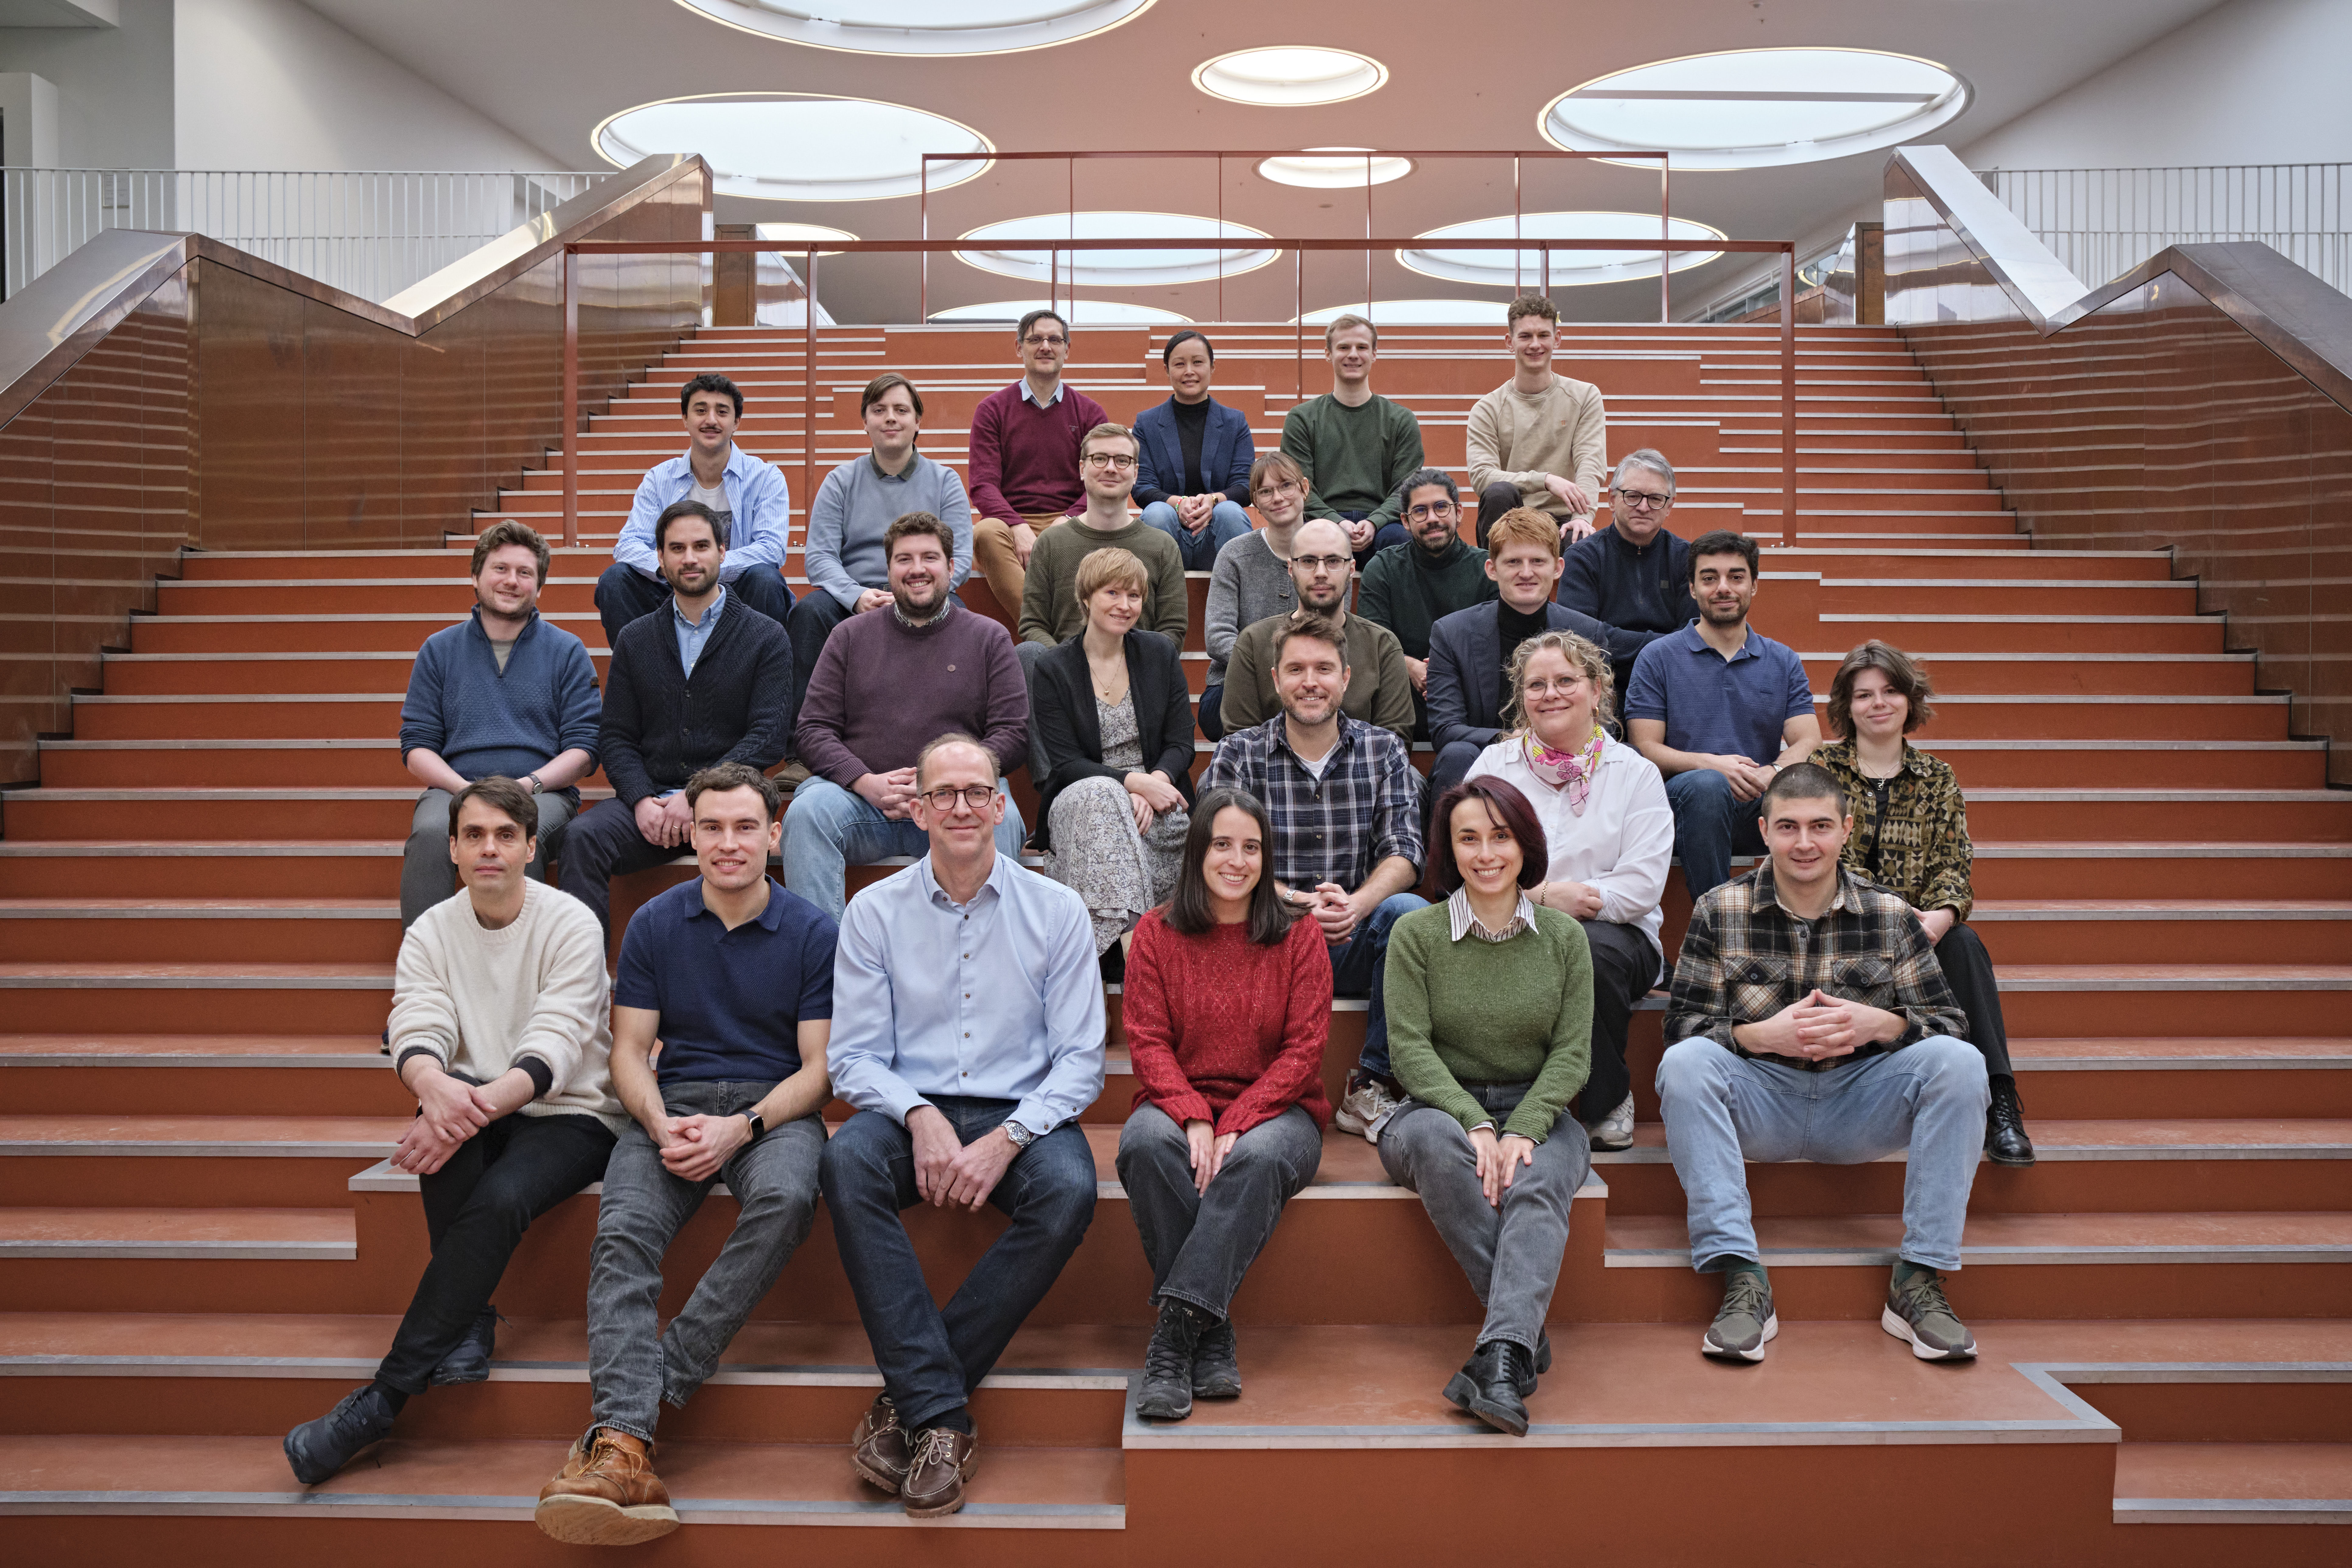
\includegraphics[scale=0.1]{Figures/POLIMA_photo.jpg}}

\end{textblock*}

\end{frame}

\end{document}